\chapter{Исследовательский раздел}
Для проверки рабоспособности алгоритмов прогнозирования на неразмеченных данных, алгоритмы проверяюлись на размеченных данных.
Информация о матчах WTA(международная женская теннистная ассоциация) за период 2007-2019 года была взята с сайта data.world\cite{Book34}, информация о матчах ATP(мужская теннисная ассоциация) была взята с сайта opendatasoft.com\cite{Book35}.
Данные о ставочных коэффициентах были взяты с сайта oddsportal.com\cite{Book36}, теннисные интервью были взяты с сайта  ASAP
Sport’s\cite{Book37}, а так же из статьи Liye Fu\cite{Book38}.В некоторых случаях в качестве предматчевого интервью использовалось послематчевое интервью предыдущего матча. Все вопросы журналистов были вырезаны из интервью. Оставлены только ответы спорсменов на вопросы журналистов Так же для корректировки статистических данных использовался портал tennis-data\cite{Book39}. Набор данных разбивался на данные для обучения и данные для тестирования в пропорции 4 к 1.
На основе сбора данных с вышеприведенных источников был сформирован датасет следующих размеров: 533 матча WTA и 1202 матча ATP.
\section{Поиск оптимального набора статистических свойств}

\begin{figure}[!h]
	\centering
	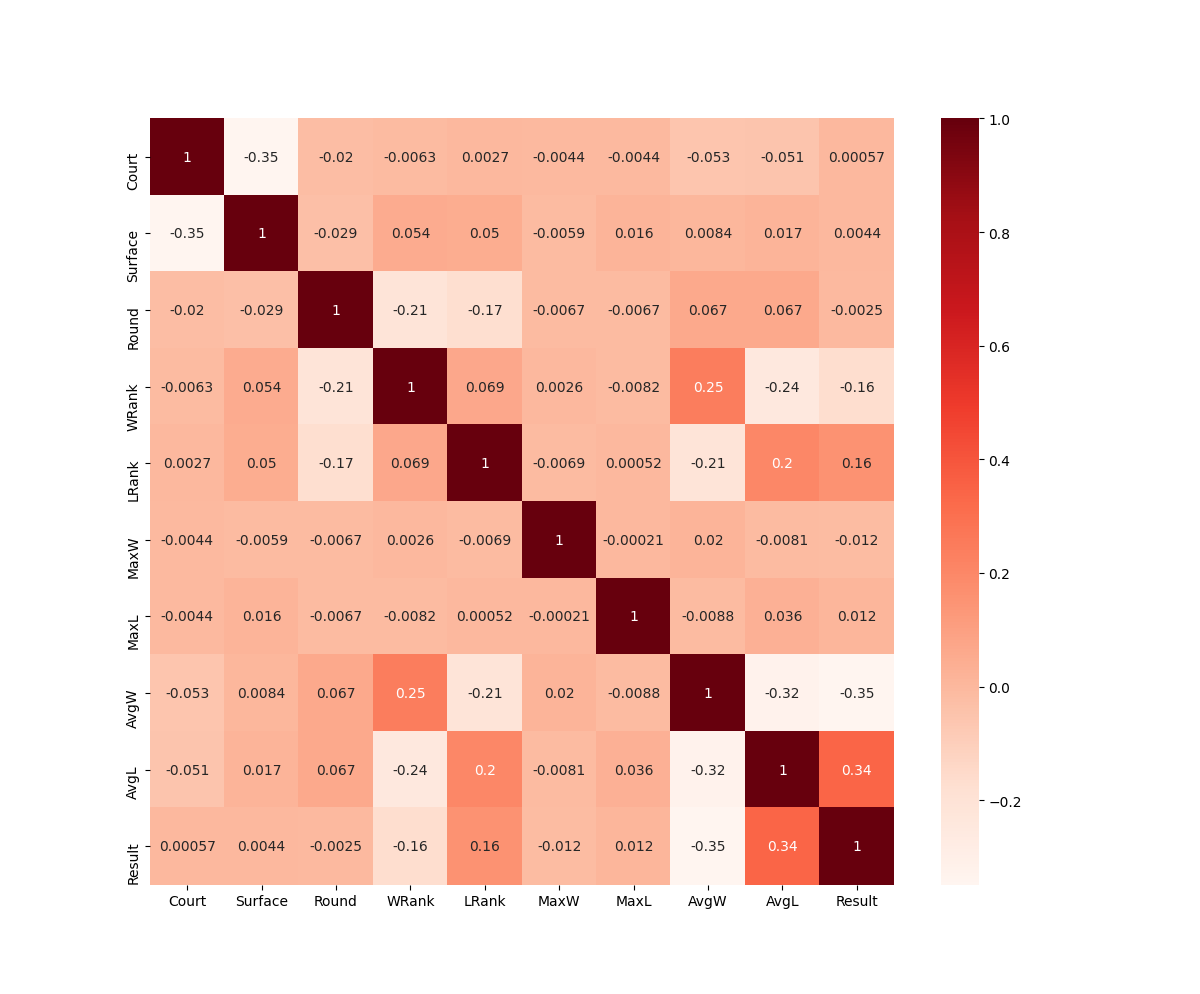
\includegraphics[width=.8\textwidth]{master_img/heatmap.png}
	\caption{Тепловая карта корреляции Пирсона}
	\label{fig03}
\end{figure}
\begin{longtable}{|l|l|}
			
			\hline
			
			Свойство& Показатель независимости \\
			
			\hline 
			
			В помещении/На улице & 0.000569 \\ \hline
			Стадия турнира & 0.002458 \\ \hline
			Покрытие корта & 0.004447 \\ \hline
			Максимальная ставка на игрока 1 & 0.011954 \\ \hline
			Максимальная ставка на игрока 2 & 0.012071 \\ \hline
			Ранг игрока 2 & 0.158269 \\ \hline
			Ранг игрока 1 & 0.164985 \\ \hline
			Cредняя ставка на игрока 1 & 0.342577 \\ \hline
			Средняя ставка на игрока 2 & 0.346160 \\ \hline

		

	\caption{Показатели независимости свойств}
	\label{tab:tablepearson}
\end{longtable}
Построим тепловую карту корреляций переменных на основе метода Пирсона(см рисунок \ref{fig03}).
На её основе отберем 5 наиболее независимых свойств в таблице \ref{tab:tablepearson}.


\section{Влияние тональности на точность прогнозов}
Была обучена и протестирована нейронная сеть с 5-ю статистическими параметрами и с 5 статистическими параметрами + 1 текстовым(итоговый вариант работы).
\begin{longtable}{|l|l|l|l|}

			
			\hline
			
			Количество свойств& Точность ATP & Точность WTA & Всего  \\
			
			\hline 
			
			5 статистических & 65.14\% & 68.86\%&  66.28\% \\ \hline
			5 стат. + тональность   & 66.40\%&72.64\% & 68.29\%   \\
			
			
			\hline
				\caption{Влияние тональности на точность прогнозов}
	\label{tab:tabletone}

	
\end{longtable}
Из полученных результатов в таблице \ref{tab:tabletone} можно заметить, что добавление столбца тональности незначительно увеличило точность прогнозов в ATP и почти на 4\% улучшилась точность прогнозов в WTA.
\bigskip
\bigskip
\pagebreak


\section{Сравнение алгоритмов прогнозирования теннисных матчей}
Сравним эффективность прогнозов полученного метода с другими аналогичными работами.
В некоторых работах не указана итоговая точность прогнозирования. Тогда точностью для данной работы считалась общее количество успешно предсказанных матчей, подёлённое на общее число проанализированных матчей\cite{Book40}. В некоторых работах не уточняется общее число проанализированных матчей.
\begin{table}[!h]
	
	\caption{\label{tab:issled1}Сравнение методов прогнозирования результатов теннисных матчей}
	
	\begin{center}
		
		\begin{tabular}{|l|l|l|l|l|}
			
			\hline
			
			Автор работы& Метод & Точность & Чис. матч.& Турниры  \\
			
			\hline 
			
			McHale и & Модель& 66.90\% & - & ATP  \\
			Morton, 2011  \cite{Book18} & Бредли-Терри& & &  \\
			\hline
			Scheibehenne и  & Агрегирование  & 70.06\% & 127 & ATP  \\
			Bröder,
			2007\cite{Book40} &рейтингов игроков&&& \\
			\hline
			Knottenbelt, Spanias,& Иерархическая & 69.38\% & 686& ATP  	\\		Madurska, 2012\cite{Book41} & модель Маркова& && \& WTA \\
			\hline
			Gu, Saaty,2019\cite{Book42} &Метод аналатич.& 85.10\%&94&ATP \\
			&сетей&&&\& WT\\
			\hline
			Метод данной &Нейронные сети& 68.29\%&347&ATP \\
			работы &&&&\& WTA\\
			\hline
		\end{tabular}
		
	\end{center}
	
\end{table}
 Из нижеприведенных данных можно заметить, что точность прогнозов уменьшается с увеличением количества аналазируемых данных.

Сравним эффективность прогнозов полученного метода с другими аналогичными работами.
В некоторых работах не указана итоговая точность прогнозирования. Тогда точностью для данной работы считалась общее количество успешно предсказанных матчей, подёлённое на общее число проанализированных матчей\cite{Book40}. В некоторых работах не уточняется общее число проанализированных матчей.
	
\begin{table}[!h]
	\begin{center}
		\begin{tabular}{|l|l|l|l|l|}
			\hline
			
			Автор работы& Точность  & Точность&ATP кол-во  & WTA кол-во \\
			& ATP & WTA&матчей. & матчей \\
			\hline 
			
			McHale и &66.90\%& - & - & -  \\
			Morton, 2011  \cite{Book18} & & & &  \\
			\hline
			Scheibehenne и  & 70.06\% & - & 127 & -  \\
			Bröder,
			2007\cite{Book40} &&&& \\
			\hline
			Knottenbelt, Spanias,& 70.30\% & 68.75\% & 270& 416	\\		Madurska, 2012\cite{Book41} & & && \\
			\hline
			Gu и  &87.4\%& 80.6\%&66&31\\
			Saaty,2019\cite{Book42}&&&&\\
			\hline
			&&&&\\
			Метод данной &66.40\%& 72.64\%&241&106\\
			работы &&&&\\
			\hline
			
			
		\end{tabular}
	\end{center}
	\caption{Сравнение методов прогнозирования результатов теннисных матчей с разбивкой по ассоциацям}		
	\label{tab:issled2}
\end{table}


Исходя из полученных результатов метрик точности для различных ассоциаций в таблице \ref{tab:issled2}, можно рекомендовать использовать данный метод в для прогнозирования турниров WTA и в некоторых случаях для прогнозирования турниров ATP.
%%% Local Variables:
%%% mode: latex
%%% TeX-master: "rpz"
%%% End: